

\subsection{Players and system model}
The formal model of the satellite system will be divided into three Markov Decision Process (MDP) player models scheduled using a non-player module. The environment player, denoted by \emath{\mathcal{P}_{env}}, encapsulates the failure states, including both scheduled maintenance and unscheduled interruptions. The model is presented in \lst{CSGSatteliteModel}. The environment player encapsulates five commands: Lines 4 and 5 trigger an interruption in the normal state with probability \emath{1-e^{mtbf/t_{\alpha}}} (where MTBF is the mean time between failures and \emath{t_{\alpha}} is a temporary unavailability). Line 6 triggers a failure according to the satellite's reliability (\emath{1 - r}, where \emath{r} represents reliability). Both scheduled and unscheduled interruptions transition the satellite system back to its normal state. However, in case of failure, the reset is synchronized with the completion (success or termination) of maneuvers by ground or on-orbit staff.

\lstdefinestyle{framed}
{
	frame=lrb,         
	mathescape,
	numbers=left,
	belowcaptionskip=-1pt,
    xleftmargin=3.11em,
		xrightmargin=0.03cm,
    framexleftmargin=3em,
	framexrightmargin=0pt,
	framextopmargin=5pt,
	framexbottommargin=5pt,
	framesep=0pt,
	rulesep=0pt,
	numbers=left,
}
    
%\lstset{breaklines=true,style=framed,escapeinside={<@}{@>},
%	morekeywords={void, int, public,private,class,protected, submodules, network,connections, const, init,int,,bool, double, module,rewards,endrewards, endmodule},basicstyle=\scriptsize\ttfamily, keywordstyle=\bfseries\color{eminence}, 
%	morecomment=[f][\color{forestgreen}][0]{/*},
%    label=queueemodel
%}
\lstset{
    breaklines=true,
    style=framed,
    escapeinside={<@}{@>},
    morekeywords={void, int, public, private, class, protected, submodules, network, connections, const, init, int, bool, double, module, rewards, endrewards, endmodule},
    basicstyle=\scriptsize\ttfamily,
    keywordstyle=\bfseries\color{blue},
    morecomment=[f][\color{green!70!black}][0]{/*},
        morecomment=[l][\color{green!30!black}]{//},
    label=queueemodel
}


\begin{figure}[!htb]            
\begin{minipage}{9cm}
\begin{lstlisting}[style=framed,%customc,
	caption=Satellite Environmental Failure Model ,
 	label=CSGSatteliteModel]	
module connector
s3: [0..3] init 0;//0 NORMAL, 1 FAILURE, 2 SCHEDULED, 3 UNSCHEDULED
//interruptions and failures commands
[Scheduled]   s3=NORMAL ->  pow(exp,-mod(z,mtbf)/talpha):(s3'=NORMAL)	+(1-pow(exp,-mod(z,mtbf)/talpha)):(s3'=SCHEDULED) ;
[Unscheduled] s3=NORMAL ->  pow(exp,-mod(z,mtbf)/talpha):(s3'=NORMAL)+(1-pow(exp,-mod(z,mtbf)/talpha)):(s3'=UNSCHEDULED) ;
[Failure]     s3=NORMAL ->  r:(s3'=NORMAL )	+(1-r):(s3'=FAILURE) ;
[Normal]      s3=NORMAL | s3=SCHEDULED | s3=UNSCHEDULED-> (s3'=NORMAL);
[Reset]      s3=Failure-> (s3'=NORMAL);
endmodule
\end{lstlisting}
 \end{minipage}  
\end{figure}

The On-orbit player model, denoted by \emath{\mathcal{P}_{o}}, is detailed in \lst{CSGSatteliteModelOnOrbitManoeuvers}. The model encapsulates four commands that interpret global behavior from \fig{fig:usecase}. The first command (line 5) models a software update that transitions the satellite from standby status to update by modifying the variable \emath{s2.}A successful update is modeled by the command in line 8 with probability \emath{e^{mtbf/mttr}} (where MTTR represents the mean time to repair). In the worst case, ground control checks the satellite's availability and replaces it with probability \emath{P_{\beta}} (line 14). Upon successful update or failure, the satellite resets to standby (line 13).
  

\begin{figure}[!htb]            
\begin{minipage}{9cm}
\begin{lstlisting}[style=framed,%customc,
	caption=OnOrbit Satellite Manoeuvers,
 	label=CSGSatteliteModelOnOrbitManoeuvers]	
module OnOrbitManoeuvers
// State variable declaration with initial value
s2: [0..10] init 0;  // s2 is an integer variable ranging from 0 to 10, initialized to 0
// State transition - repair on-orbit software update
[RepairOnOrbitSoftwareUpdate]   	// Label for the transition
s2=STANDBY -> (s2'=UPDATE);       // The system transitions from standby (s2=STANDBY) to update state (s2'=UPDATE) for software update
// State transition - check for redundant satellite (from update state)
[CheckOnOrbitRedundantSatellite]        s2=UPDATE  -> (1-pow(exp,-mod(z,mtbf)/tmttr)):(s2'=CHECKSATTELITE)+(pow(exp,-mod(z,mtbf)/tmttr)):(s2'=STANDBY) ;
// State transition - move/replace redundant satellite (from check state)
[MoveReplaceRedundantSatellite]         s2=CHECKSATTELITE           -> Pbeta:(s2'=REPLACE)+(1-Pbeta):(s2'=ONGROUNDSPARE);
// State transition - reset to standby
[ResetOnOrbitManoeuvers]       		// Label for the transition
s2=ONGROUNDSPARE | s2=REPLACE | s2=UPDATE    -> (s2'=STANDBY);  // The system can reset to standby from various states (ONGROUNDSPARE, REPLACE, UPDATE) and sets s2' (next state) to standby
endmodule
\end{lstlisting}
 \end{minipage}  
\end{figure}

The On-ground player model, denoted by \emath{\mathcal{P}_{g}}, is detailed in  \lst{CSGSatteliteModelOnGroundManoeuvers}. The model encapsulates five commands that interpret global on-ground behavior from \fig{fig:usecase}. The first command (line 5) models a staff member transitioning the satellite from standby status to on-ground spare by modifying the variable \emath{s1}. Building a new satellite is modeled by the command in line 6 with probability \emath{1-e^{mtbf/t_{\gamma}}}(where \emath{t_{\gamma}}represents the mean-time to build a satellite). In this case, ground control initiates preparations for launching the new satellite. When the satellite is built (line 8, taking \emath{t_{\delta}} time), they prepare it for launch (line 10). Finally, when the satellite is ready for launch (line 12), the ground staff returns to standby mode with probability \emath{P_{n}}.
 

\begin{figure}[!htb]            
\begin{minipage}{9cm}
\begin{lstlisting}[style=framed,%customc,
	caption=On-Ground Satellite Manoeuvers,
 	label=CSGSatteliteModelOnGroundManoeuvers]	
module OnGroundManoeuvers
s1: [0..10] init 0; //refers to the on-ground modes
//The satellite on the ground is on standby mode
[OnGroundStandby] s1=STANDBY  -> (s1'=ONGROUNDSPARE);
//Building mode of a new satellite or initiate the launch
[CheckOnGroundSatelliteToBuild] s1=ONGROUNDSPARE  -> (1-pow(exp,-mod(z,mtbf)/tgamma)):(s1'=BUILD)+(pow(exp,-mod(z,mtbf)/tgamma)):(s1'=LAUNCH);
//build a new satellite or fail and  standby mode
[CheckOnGroundSatelliteToManufecture]   s1=BUILD  -> (1-pow(exp,-mod(z,mtbf)/tdelta)):(s1'=MANUFECTURE)+(pow(exp,-mod(z,mtbf)/tdelta)):(s1'=STANDBY);
// When the satellite is manufactured launch it
[BuildOnGroundSatellite] s1=MANUFECTURE    -> (s1'=LAUNCH);
//reset the on-ground operations
[ResetOnGroundManoeuvers] s1=LAUNCH -> (1-Pn):(s1'=LAUNCH)+(Pn):(s1'=STANDBY);
endmodule
\end{lstlisting}
 \end{minipage}  
\end{figure}

\paragraph{Experimental setup} We have encoded properties in rPATL formalism. PRISM-games model checker 3.0 \cite{Kwiatkowska2020} performs probabilistic verification. These experiments were conducted on a Ubuntu-I7 system equipped with 32GB RAM. Multiple engines can be selected (refer to documentation \cite{engines}) offering performance benefits for specific model structures. 

\paragraph{Artifacts} The source code for the experiments described in this section is publicly available on a GitHub repository\cite{seaa2024}. %The website provides comprehensive instructions on how to replicate the experiments.


\subsection{Properties of the modeled system as game goals}


We have identified the need to analyze satellite systems' reliability, availability, and maintainability (RAM) properties. Reliability refers to the satellite's ability to function without failures, considering scheduled and unscheduled interruptions. Maintainability reflects the ease with which the satellite can be repaired, with in-orbit repair being a key aspect.  The PRISM-games tool provides support for automated analysis of properties expressed in rPATL. So we express the system properties in natural language and then map them to the rPATL structure:

\subsubsection{\underline{Reliability}} 

\emph{What is the probability that a satellite will need to be replaced by a new one in 15 years, given a reliability of 0.80 regarding failures within 30 attempts?}

	   
	    \begin{resp}{}
             \begin{equation}
             \splitdfrac{\mathtt{  \langle\langle\textcolor{red}{\mathcal{P}_{env}}, \textcolor{red}{\mathcal{P}_{o}}, \textcolor{red}{\mathcal{P}_{g}}} \rangle\rangle}{ \\ \mathtt{ P=? [ F \ (\quot{\textcolor{red}{replace}} \ \& \ \textcolor{red}{rounds}<=\textcolor{red}{k}) ] ,k=\textcolor{blue}{1:30:1}}} 
        \label{eq1}
        \tag{PRO1}
    \end{equation}
        \end{resp}
        \normalsize

\subsubsection{\underline{Maintainability}} \emph{How many times would a satellite need to be replaced by a new one in 15 years, assuming a reliability of 0.80 regarding failures within 30 attempts?}

	   
	    \begin{resp}{ }
             \begin{equation}
             \splitdfrac{\mathtt{  \langle\langle\textcolor{red}{\mathcal{P}_{env}}, \textcolor{red}{\mathcal{P}_{o}}, \textcolor{red}{\mathcal{P}_{g}}} \rangle\rangle}{ \\ \mathtt{ R\{\quot{\textcolor{red}{replace}} \}=? [ F \  (\textcolor{red}{rounds}<=\textcolor{red}{k}) ] ,k=\textcolor{blue}{1:30:1}}} 
        \label{eq2}
        \tag{PRO2}
    \end{equation}
        \end{resp}
        \normalsize

\subsubsection{\underline{Availability}} \emph{What is the availability of the satellite in 15 years, assuming a reliability of 0.80 regarding failures within 30 attempts?}. We use T as a reference to the maximum number of rounds (attempts) to reach a successful replacement.

    \begin{resp}{ }
             \begin{equation}
             \splitdfrac{\mathtt{  \langle\langle\textcolor{red}{\mathcal{P}_{env}}, \textcolor{red}{\mathcal{P}_{o}}, \textcolor{red}{\mathcal{P}_{g}}} \rangle\rangle}{ \\ \mathtt{ R\{\quot{\textcolor{red}{replace}} \}=? [ F \  (\textcolor{red}{rounds}<=\textcolor{red}{k}) ]/T ,k=\textcolor{blue}{1:30:1}}} 
        \label{eq3}
        \tag{PRO3}
    \end{equation}
        \end{resp}
        \normalsize

\subsubsection{\underline{Maintenance cost}} \emph{What is the cost of the satellite replacement in 15 years, assuming a reliability of 0.80 regarding failures within 30 attempts?} 

    \begin{resp}{ }
             \begin{equation}
             \splitdfrac{\mathtt{  \langle\langle\textcolor{red}{\mathcal{P}_{env}}, \textcolor{red}{\mathcal{P}_{o}}, \textcolor{red}{\mathcal{P}_{g}}} \rangle\rangle}{ \\ \mathtt{ R\{\quot{\textcolor{red}{cost}} \}=? [ F \  (\textcolor{red}{rounds}<=\textcolor{red}{k}) ] ,k=\textcolor{blue}{1:30:1}}} 
        \label{eq4}
        \tag{PRO4}
    \end{equation}
        \end{resp}
        \normalsize

To address the properties mentioned above, we propose extending the model with a module to track the number of rounds synchronized with module actions. Additionally, we will incorporate a reward structure to model replacement times and costs.
        
First, we enhance the model by incorporating an integer constant as in \cite{KNPS19} and a module (see \lst{lst:rounds}) to keep track of the number of rounds. In this case, as the commands are unaffected by the players' choices, they are considered unlabeled with empty action. Consequently, these commands are executed regardless of the actions taken by the players. Furthermore, the module is deterministic due to the disjoint guards present in both commands. 

\begin{figure}[htbp]            
\begin{minipage}{9cm}
\begin{lstlisting}[style=framed,%customc, 
caption=Rounds Module,
 	label=lst:rounds]	
const k; // number of rounds
module rounds // module to count the rounds
 rounds : [0..k+1];
 [] rounds<=k -> (rounds'=rounds+1);
 [] rounds=k+1 -> true;
endmodule
\end{lstlisting}
 \end{minipage}  
\end{figure}

Second, we define five reward structures in \lst{lst:cost}. These structures correspond to the replacement times for in-orbit and on-ground operations (lines 3-6). They are divided into separate reward structures for in-orbit and on-ground replacements (lines 7-12). The cost of these replacements is modeled in lines 13-18. Here, c1 represents the cost of replacing a satellite in orbit, while c2 represents the cost of manufacturing a new satellite on the ground. \emph{Properties in \ref{eq2} and \ref{eq4} with tag name \quot{replace} and \quot{cost} can be replaced with on-orbit and on-ground replace and cost as rewards names in \lst{lst:cost}}.

\begin{figure}[htbp]            
\begin{minipage}{9cm}
\begin{lstlisting}[style=framed,%customc, 
caption=Reward Structures in PRISM,
 	label=lst:cost]	
const double c1; //Cost of replacing a satellite in orbit
const double c2; //Cost of manufacturing a new satellite on the ground
rewards "replace" // Reward for replacing a satellite on ground and on-orbit
  s2=REPLACE : 1;  // Replace satellite with a new one
  s1=MANUFECTURE : 1; // Manufacture a new satellite to replace satellite 
endrewards
rewards "replaceOnOrbit" // Reward for replacing a satellite on orbit
  s2 = REPLACE : 1; // Replace satellite with a new one
endrewards
rewards "replaceOnGround" // Reward for replacing a satellite on ground
  s1 = MANUFACTURE : 1; // Manufacture a new satellite to replace satellite 
endrewards
rewards "costOnOrbit" // Cost of replacing a satellite on orbit
  s2 = REPLACE : c1 * rounds; // Replace satellite with a new one, incurring a cost proportional to rounds
endrewards
rewards "costOnGround" // Cost of replacing a satellite on ground
  s1 = MANUFACTURE : c2 * rounds; // Manufacture a new satellite to replace satellite, incurring a cost proportional to rounds
endrewards
\end{lstlisting}
 \end{minipage}  
\end{figure}

\subsection{Experiments results analyses}

\noindent
   \begin{figure*}[htbp]
       \begin{tabularx}{\linewidth}{m{8cm}  m{8cm}}
 

 \begin{minipage}[t]{8cm}
     \centering

    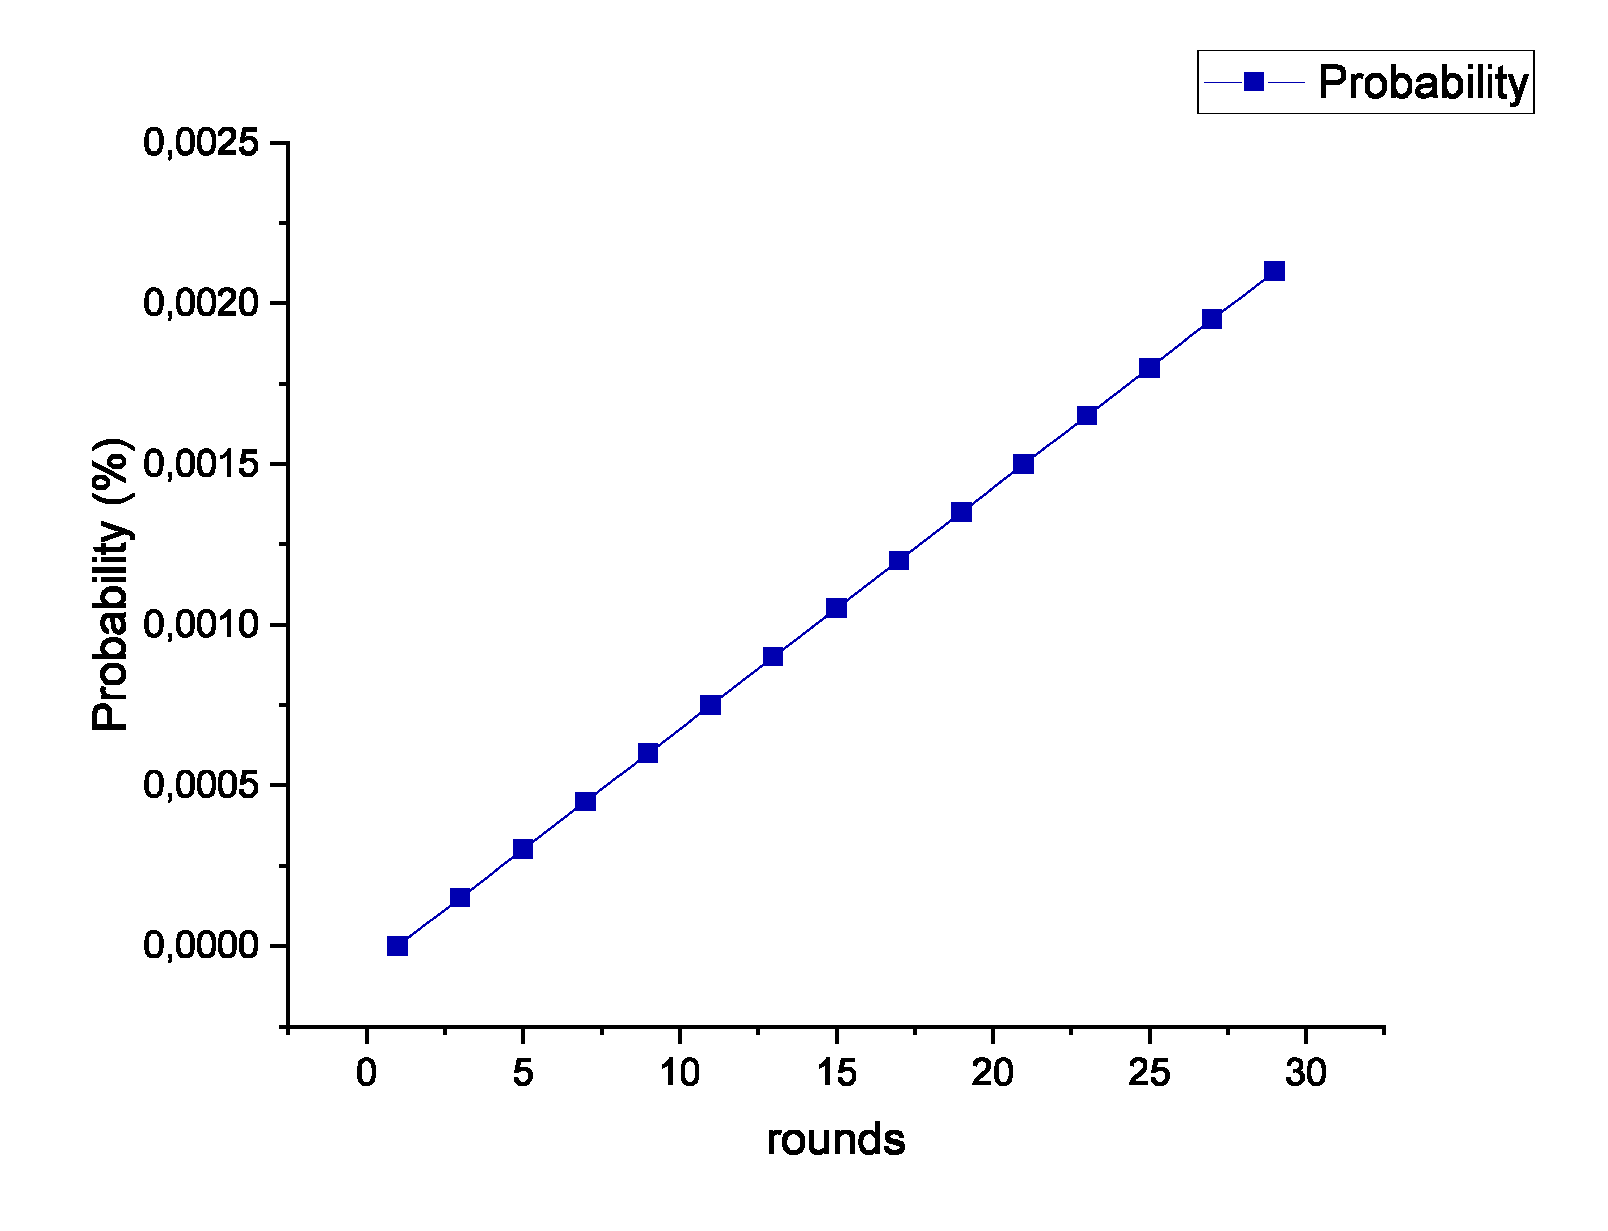
\includegraphics[width=170pt, height =135pt]{Graph01.pdf}
    \caption{Verif. \ref{eq1} .}
    \label{fig:1}
   \end{minipage}
    
           &
           

 \begin{minipage}[t]{8cm}
     \centering

    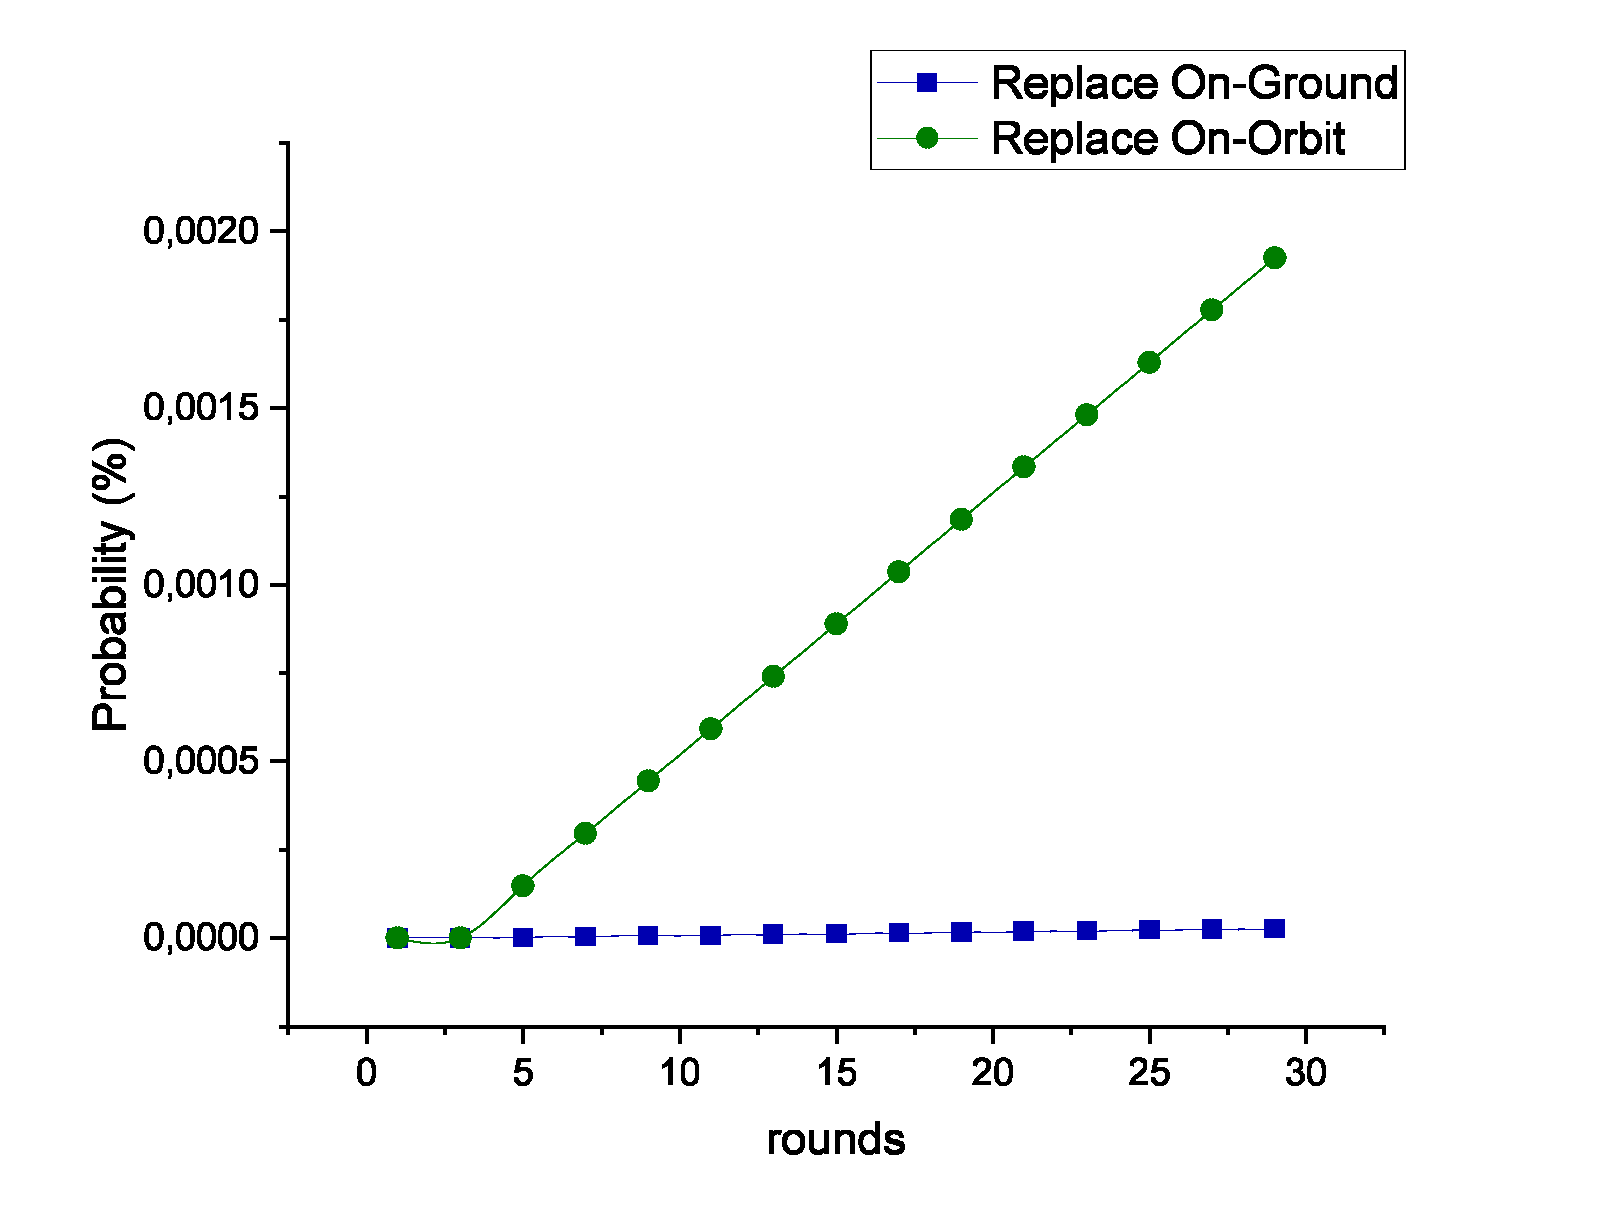
\includegraphics[width=170pt, height =135pt]{Graph02.pdf}
    \caption{Verif. \ref{eq2}.}
    \label{fig:2}
   \end{minipage}
    

       \\ 
   \begin{minipage}[t]{8cm}
     \centering

    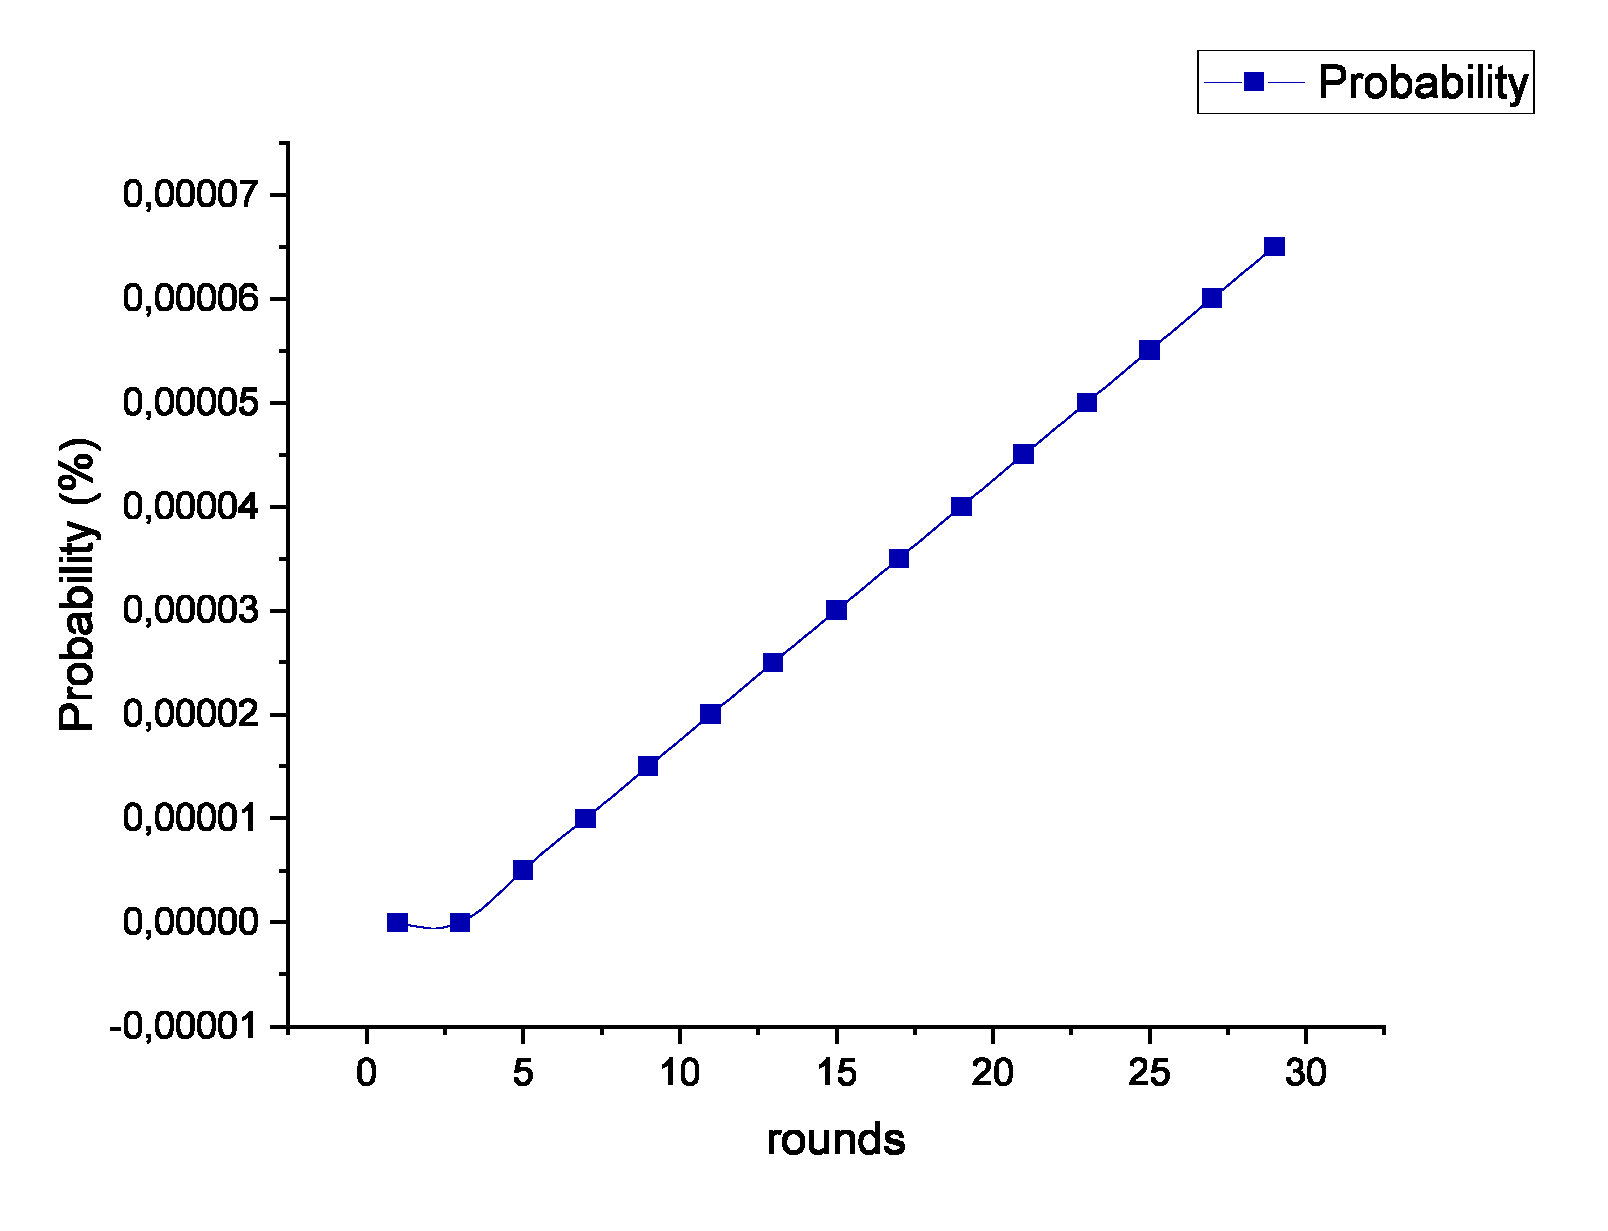
\includegraphics[width=170pt, height =135pt]{Graph03.pdf}
    \caption{Verif. \ref{eq3} .}
    \label{fig:3}
   \end{minipage}
    
           &
           

 \begin{minipage}[t]{8cm}
     \centering

    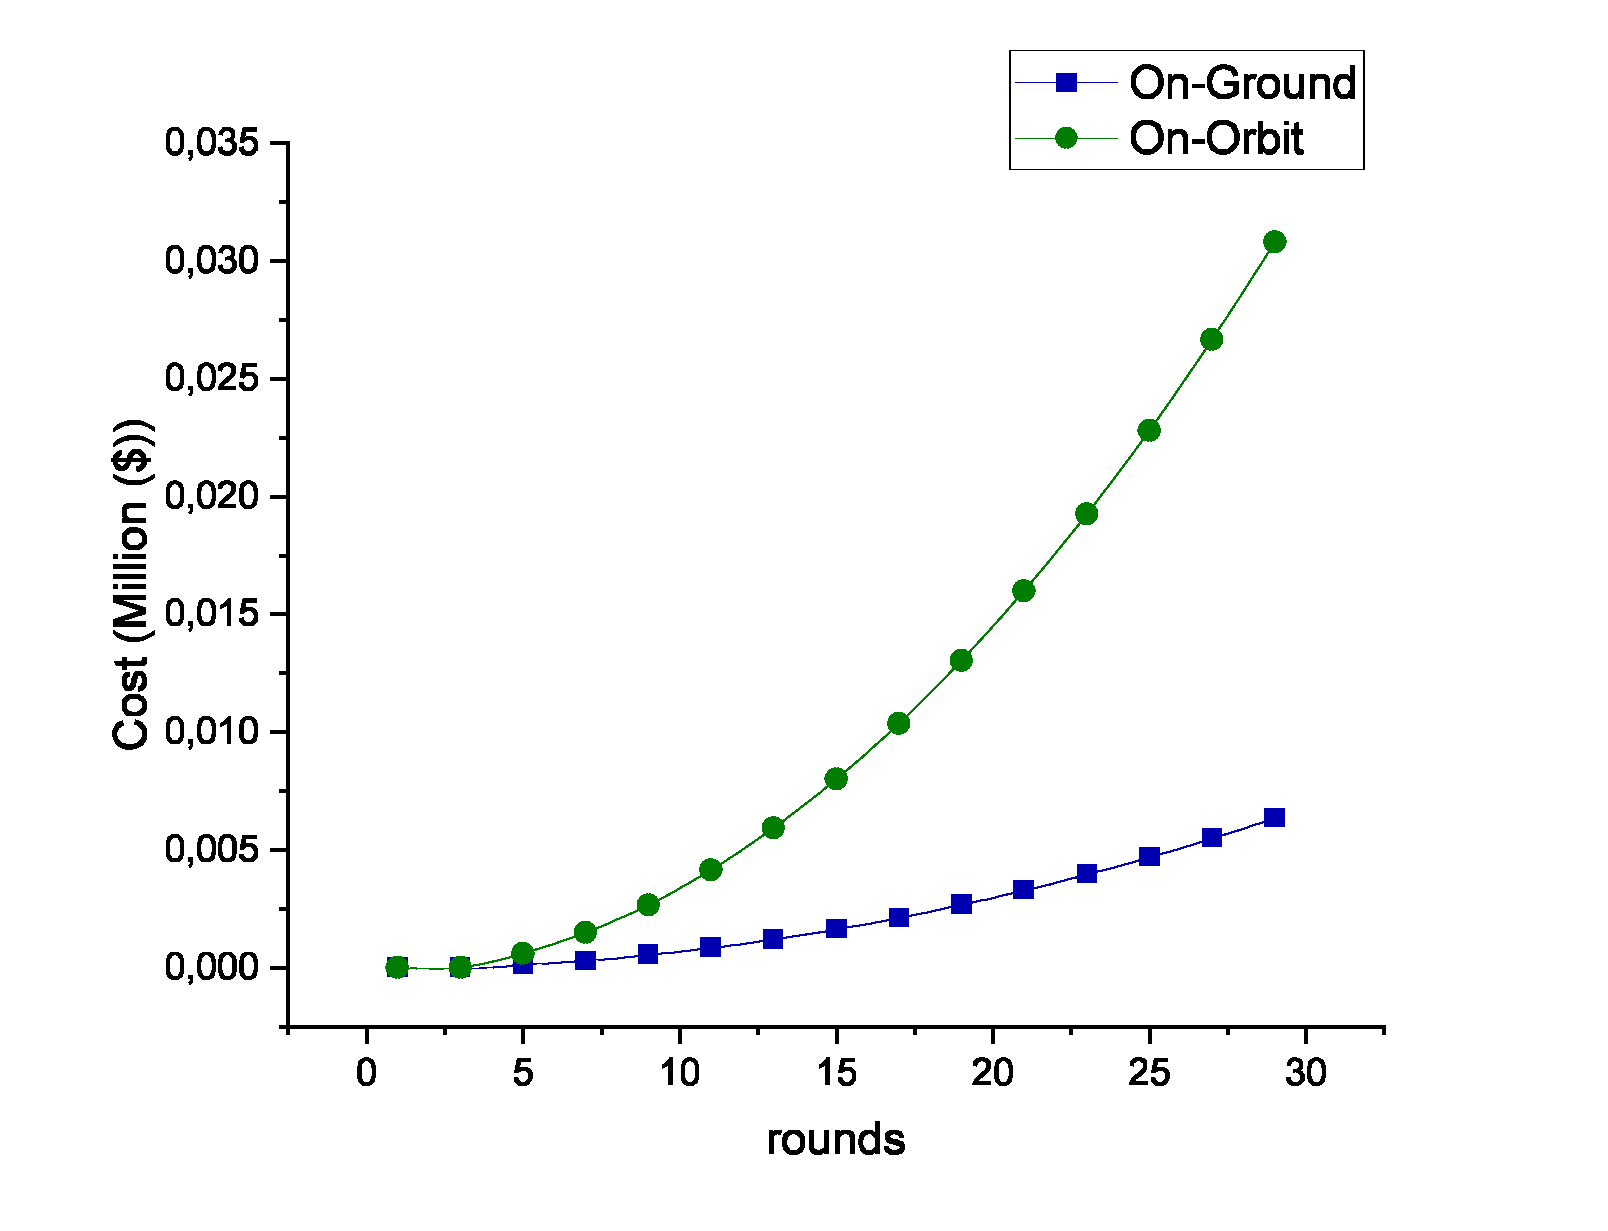
\includegraphics[width=170pt, height =135pt]{Graph04.pdf}
    \caption{Verif. \ref{eq4}.}
    \label{fig:4}
   \end{minipage}
   
           \end{tabularx}
\end{figure*}

The verification results for \ref{eq1} are shown in \fig{fig:1}. We observe that as the number of rounds increases, the probability of replacement for satellites in orbit or on the ground also increases. This is likely because the staff are more willing to replace satellites in multiple rounds to ensure maximum functionality and avoid failures throughout their 15-year lifespan.

The verification results for \ref{eq2} are shown in \fig{fig:2}. As the number of rounds increases, the probability of replacing both on-orbit and ground satellites also increases. However, on-orbit maintenance is more frequent than ground maintenance. This is due to the higher cost of manufacturing and launching a new satellite. Consequently, on-orbit staff tend to prioritize repairing existing satellites or finding spare ones in orbit whenever possible.

The verification results for \ref{eq3} are shown in \fig{fig:3}. We observe that the availability of the satellite increases. This can be interpreted as an increase in the satellite replacement rate as the number of rounds increases. This strategy aims to maximize the satellite's availability after 30 rounds. However, it's important to note that the maximum achievable replacement rate is equivalent to 0.008\%, which represents the limit of the staff's effort.


The verification results for Equation \ref{eq4} are shown in \fig{fig:4}. These results indicate that on-orbit staff maintenance incurs a cost of \$0.035 million more than on-ground maintenance. This is because staff prioritize on-orbit replacements over ground replacements. Interestingly, our initial assumption was that on-ground maintenance would be more expensive than on-orbit maintenance. However, the actual cost depends on the total number of replacements performed (as shown in \fig{fig:4}). This suggests that on-ground staff can develop a maintenance strategy that achieves higher satellite availability in fewer rounds, even though this strategy might require a larger initial maintenance budget.

\subsection{Threats to validity}
Our model currently focuses on a single satellite system. (i) For scenarios involving multiple cooperating satellites, additional staff collaboration would be necessary for repairs and maintenance, potentially introducing a first-in-first-out (FIFO) queueing system.  Furthermore, the maintenance parameters may change. (ii) The model does not consider communication between the ground station and the satellite system, which factors like solar radiation can impact. (iii) The interaction between on-orbit and ground staff has not been explicitly modeled in our current approach. However, their collaboration can significantly impact the maintenance strategy like the team size and involvement cost.


\subsection{Discussion}


Strategic maintenance implementation can enhance the quality of a satellite system while optimizing failure repair. The model can be extended with additional commands to simulate communication. Our current focus is on existing commands implemented by our collaborators and researchers.

The model is parametric, allowing for customization using different parameters within the PRISM-games. The data employed aligns closely with the models described in  \cite{Hoque2015,Yu2015}. However, a key difference lies in the model formalism. Previous implementations relied on CTMC and MDPs, whereas this work leverages the CSG formalism to include the human response. To our knowledge, this is the first implementation using CSGs for RAM analysis in satellite systems with collaborative maintenance (based on the PRISM library \cite{prismgames}).

Failures are primarily modeled using an exponential distribution. Additional distributions can be incorporated through appropriate model updates, reflecting the failure distribution of specific components.
